\section{HTML Templates}\label{html-templates}

\begin{itemize}
\item
  TODO:
\item
  Ausformulieren:
\item
  Complete
\end{itemize}

\subsection{Einführung}\label{einfuxfchrung}

\begin{itemize}
\tightlist
\item
  Templates für Code sind bisher nur im Backend verfügbar in PHP oder
  Ruby z.B.
\item
  Erhält Einzug in den Browser
\item
  Bisher durch Mustache.js oder Handlebars.js
\end{itemize}

\subsection{Bisherige templatetisierung im
Browser}\label{bisherige-templatetisierung-im-browser}

\subsubsection{Via hidden div-Element}\label{via-hidden-div-element}

\begin{Shaded}
\begin{Highlighting}[]
\KeywordTok{<div}\OtherTok{ id=}\StringTok{"mydivtemplate"}\OtherTok{ style=}\StringTok{"display: none;"}\KeywordTok{>}
  \KeywordTok{<div>}
    \KeywordTok{<img}\OtherTok{ src=}\StringTok{"myimage.jpg"}\KeywordTok{>}
  \KeywordTok{</div>}
\KeywordTok{</div>}
\end{Highlighting}
\end{Shaded}

\emph{Nachteil:} - Resources werden geladen, auch wenn man sie nicht
braucht, da sie ja nicht angezeigt werden sollen - Resourcen und
Performance Verschwendung - Schwieriges Stylen und Themen. Eine Seite
die das Template verwendet muss alle CSS Regeln für das Template mit
\texttt{\#mydivtemplate} erstellen

\subsubsection{Via script-Element:}\label{via-script-element}

\begin{Shaded}
\begin{Highlighting}[]
\KeywordTok{<script}\OtherTok{ type=}\StringTok{"text/template"}\KeywordTok{>}
  \OperatorTok{<}\NormalTok{div}\OperatorTok{>}
    \OperatorTok{<}\NormalTok{img src}\OperatorTok{=}\StringTok{"myimage.jpg"}\OperatorTok{>}
  \OperatorTok{<}\SpecialStringTok{/div>}
\SpecialStringTok{</script}\OperatorTok{>}
\end{Highlighting}
\end{Shaded}

\emph{Nachteil:} - Sicherheit: Das Template wird via \texttt{innerHTML}
in einen DOM konvertiert, was eine Cross Site Scripting Sicherheitslücke
darstellen kann

\subsection{\texorpdfstring{\texttt{\textless{}template\textgreater{}}
Tag}{\textless{}template\textgreater{} Tag}}\label{template-tag}

\begin{Shaded}
\begin{Highlighting}[]
\KeywordTok{<template}\OtherTok{ id=}\StringTok{"mytemplate"}\KeywordTok{>}
  \KeywordTok{<style>}
    \CommentTok{/* Styles */}
  \KeywordTok{</style>}
  \KeywordTok{<script>}
    \CommentTok{// JavaScript}
  \KeywordTok{</script>}
  \KeywordTok{<img}\OtherTok{ src=}\StringTok{""}\KeywordTok{>} \CommentTok{<!-- Kann zur Laufzeit dynamisch gesetzt werden -->}
  \KeywordTok{<div}\OtherTok{ class=}\StringTok{"text"}\KeywordTok{></div>}
\KeywordTok{</template>}
\end{Highlighting}
\end{Shaded}

\subsubsection{Benutzung}\label{benutzung}

\begin{itemize}
\tightlist
\item
  Im Quelltext steht an beliebiger Stelle ein
  \texttt{\textless{}template\textgreater{}}-Tag
\item
  Der \texttt{template}-Knoten des DOM wird ausgewählt (1)
\item
  Der ``content'', also der Inhalt des
  \texttt{\textless{}template\textgreater{}} wird geklont (2) und an
  einer anderen Stelle im DOM wieder eingefügt (3)
\end{itemize}

\begin{Shaded}
\begin{Highlighting}[]
\KeywordTok{var} \NormalTok{template }\OperatorTok{=} \VariableTok{document}\NormalTok{.}\AttributeTok{querySelector}\NormalTok{(}\StringTok{'#mytemplate'}\NormalTok{)}\OperatorTok{;}             \CommentTok{// (1)}
\KeywordTok{var} \NormalTok{templateClone }\OperatorTok{=} \VariableTok{document}\NormalTok{.}\AttributeTok{importNode}\NormalTok{(}\VariableTok{template}\NormalTok{.}\AttributeTok{content}\OperatorTok{,} \KeywordTok{true}\NormalTok{)}\OperatorTok{;}  \CommentTok{// (2)}
\VariableTok{document}\NormalTok{.}\VariableTok{body}\NormalTok{.}\AttributeTok{appendChild}\NormalTok{(templateClone)}\OperatorTok{;}                         \CommentTok{// (3)}
\end{Highlighting}
\end{Shaded}

\subsubsection{Vorteile}\label{vorteile}

\begin{itemize}
\tightlist
\item
  Templates sind ein fertiges Gerüst an HTML
\item
  Templates werden in DOM geladen, aber nicht angezeigt bis sie
  aktiviert werden
\item
  \texttt{\textless{}script\textgreater{}} Tags werden nicht ausgeführt,
  Stylesheets/Bilder nicht geladen, Medien nicht abgespielt, bis das
  Template benutzt wird
\item
  Es können beliebig viele \texttt{\textless{}template\textgreater{}}
  Tags benutzt werden, ohne dass sich die Performance signifikant
  verschlechtert
\item
  Sie können an beliebiger Stelle im Quelltext stehen, die
  \texttt{display} Eigenschaft muss nicht getoggelt werden und es
  entsteht kein Overhead an Markup das nicht vom Browser geparst wird
\item
  Sind im Dokument versteckt, man kann nicht in den DOM des
  \texttt{\textless{}templates\textgreater{}} traversieren z.B.
  \texttt{document.getElementById(\textquotesingle{}\#mytemplate\textquotesingle{})\ ==\ null}
\item
  Mit JavaScript kann auf das Template zugegriffen werden und es an
  anderer Stelle dynamisch einbinden
\item
  Es muss mit Javascript kein Code erzeugt werden, man kann ihn einfach
  aus dem DOM nehmen und wiederbenutzen
\end{itemize}

\emph{Hinweis:} Geschachtelte \texttt{\textless{}template\textgreater{}}
Tags müssen manuell aktiviert werden!

\subsection{Browserunterstützung}\label{browserunterstuxfctzung}

\begin{itemize}
\tightlist
\item
  Sind standardisiert
  (http://www.w3.org/TR/html5/scripting-1.html\#the-template-element)
  (als einzige Technologie des Web Components Technology Stacks)
\item
  Browserunterstützung dementsprechend gut, bis auf Internet Explorer
  und Edge
\end{itemize}

\begin{figure}[htbp]
\centering
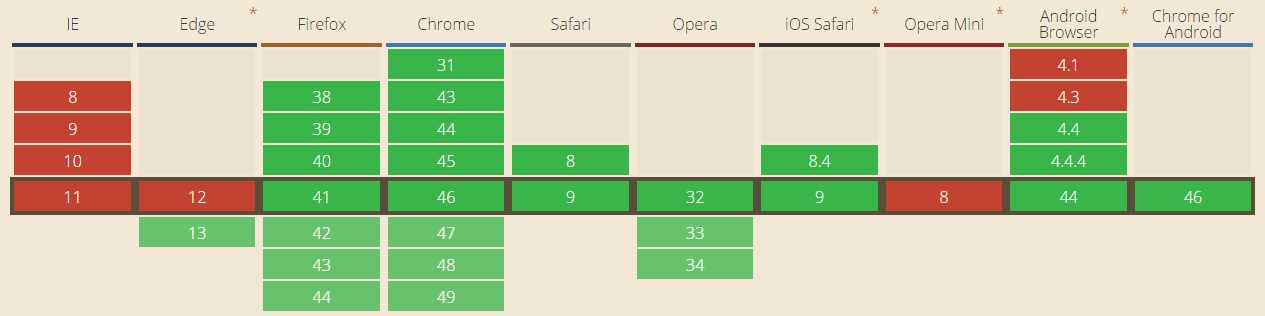
\includegraphics{images/3-html-templates-browserunterstuetzung.jpg}
\caption{Bild: Brwoserunterstützung des HTML Template Tags}
\end{figure}

\subsection{Quellen}\label{quellen}

\begin{itemize}
\tightlist
\item
  O'Reilly Buch ``Developing Web Components'', S.101-107
\item
  https://developer.mozilla.org/de/docs/Web/HTML/Element/template
\item
  http://www.html5rocks.com/en/tutorials/webcomponents/template/
\item
  http://webcomponents.org/articles/introduction-to-template-element/
\item
  http://caniuse.com/\#search=template
\item
  http://www.webcomponentsshift.com/\#13
\item
  https://frontend.namics.com/2014/03/20/web-components-html-templates-2/
\end{itemize}
